\section{Introduction}
\begin{frame}
    \frametitle{The 0/1 Knapsack Problem: Definition \& Context}

    \begin{columns}[T] % Use columns for a side-by-side layout
        
        % --- LEFT COLUMN: Two stacked images ---
        \begin{column}{0.4\textwidth}
            \begin{figure}
                \centering
                
                % First subfigure (Knapsack)
                \subfloat[The Knapsack Problem Analogy.]{
                    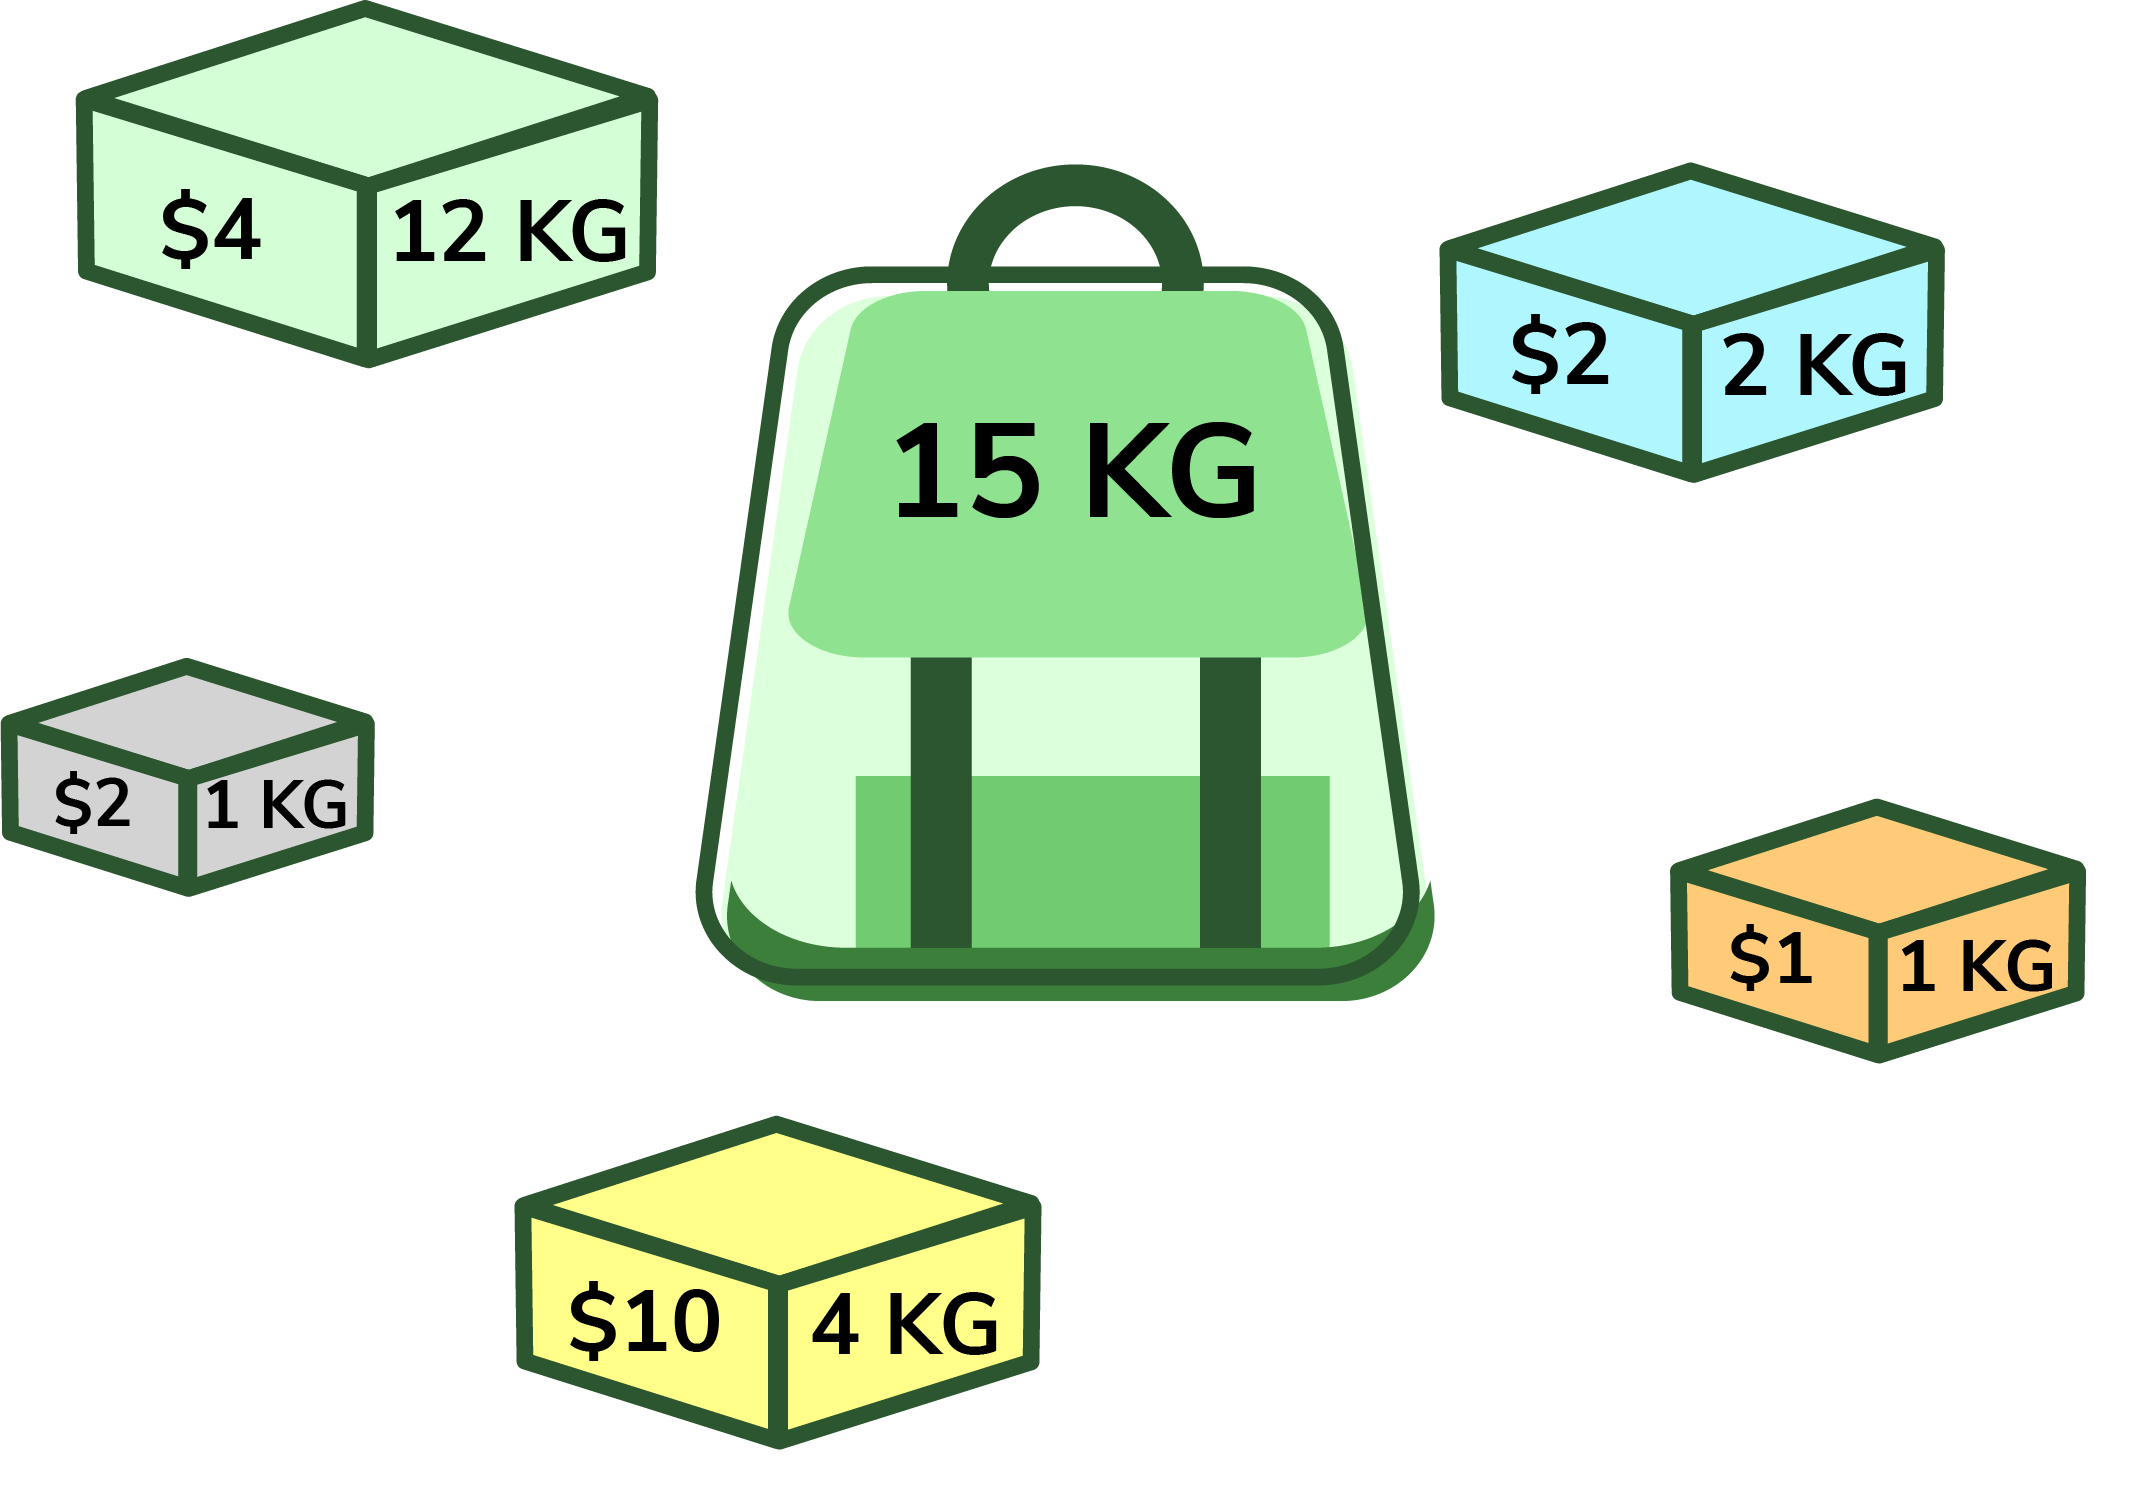
\includegraphics[width=0.9\textwidth, height=0.35\textheight]{knapsack_def.png}
                    \label{fig:knapsack_def}
                }
                
                \vspace{-1em} % Adjust space between the two images
                
                % Second subfigure (Venn Diagram)
                \subfloat[Computational Complexity Classes.]{
                    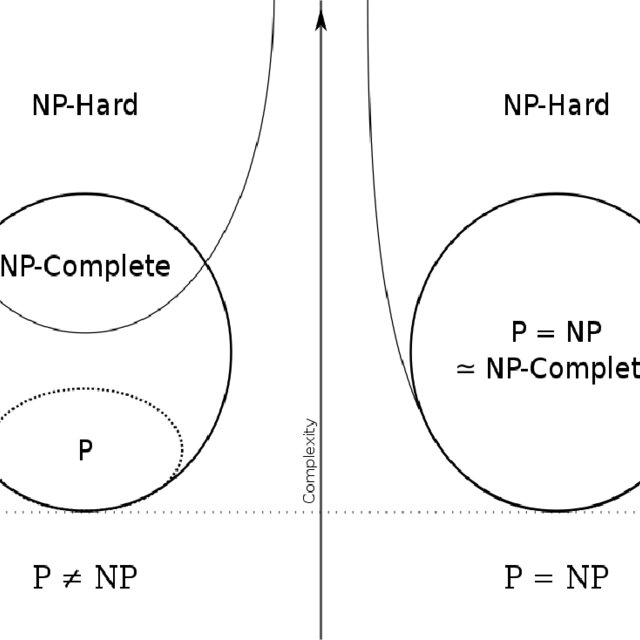
\includegraphics[width=0.9\textwidth, height=0.35\textheight]{np-venn.jpg}
                    \label{fig:np-venn}
                }
                
            \end{figure}
        \end{column}
        
        % --- RIGHT COLUMN: Definition and Importance ---
        \begin{column}{0.6\textwidth}
            
            % --- Top Part: The Definition ---
            \begin{block}{The 0/1 Knapsack Problem}
                Given $n$ items with weights and values, choose a subset.
                \begin{itemize}
                    \item \textbf{Objective:} Maximize the total value.
                    \item \textbf{Constraint:} The total weight must not exceed the knapsack's capacity.
                    \item \textbf{Rule:} Each item is either taken (1) or left (0), no fractions
                \end{itemize}
            \end{block}

            % --- Bottom Part: Context and Importance ---
            \begin{alertblock}{Applications \& Complexity}
                \begin{itemize}
                    \item \textbf{Real-world Applications:} Portfolio selection, resource allocation, logistics. \vspace{0.5em}
                    
                    \item \textbf{Problem Variants:} Many variants exist by altering constraints or item properties. The 0/1 version is the most common. \vspace{0.5em}
                    
                    \item \textbf{Computational Hardness:} KP is \textbf{NP-complete}. There is no known polynomial-time exact solution.
                \end{itemize}
            \end{alertblock}
            
        \end{column}
    \end{columns}
\end{frame}